\section{主板结构}

\subsection{芯片组}
芯片组(chipset, PC chipset, or chip set)是一组共同工作的集成电路(“芯片”),并作为一个产品销售。它负责将电脑的核心——微处理器和机器的其他部分相连接,是决定主板级别的重要部件。以往,芯片组由多颗芯片组成,慢慢的简化为两颗芯片。

在计算机领域,“芯片组”术语通常是特指计算机主板或扩展卡上的芯片,如图\ref{fig:chipset}所示。当讨论基于英特尔的奔腾级处理器的个人电脑时,芯片组一词通常指两个主要的主板芯片组:北桥和南桥。芯片组的制造商可以,通常也是独立于主板的制造商。比如PC主板芯片组包括NVIDIA的nForce芯片组和威盛电子公司的KT880,都是为AMD处理器开发的,或英特尔许多芯片组。
\begin{figure}[ht]
	\begin{center}
		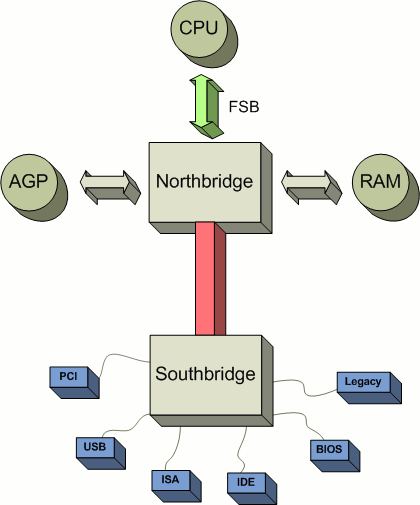
\includegraphics[keepaspectratio,width=0.5\paperwidth]{Pictures/Schema_chipsatz.png}
	\end{center}
	\caption{主板芯片组}
	\label{fig:chipset}
\end{figure}

单芯片芯片组已推出多年,例如SiS 730。但直到最近nForce 4的出现才逐渐流行。现在的单芯片芯片组,不像以往般复杂,因Athlon 64已内建内存控制器,取代了北桥的功能。纵使芯片组变成单芯片,习惯上亦沿用旧名称。

北桥(英语:Northbridge)是基于Intel处理器的个人电脑主板芯片组两枚芯片中的一枚,北桥设计用来处理高速信号,通常处理中央处理器、随机存取存储器、AGP或PCI Express的端口,还有与南桥之间的通信。


传统的北桥内建内存控制器,让处理器连接前端总线,而处理器和内存总线则跑相同的时脉。随后,芯片组分开处理器和内存总线的频率,让前端总线只代表处理器和北桥之间的通道。

北桥留下来的只剩下AGP或PCI Express控制器和与南桥通信,有时北桥会和南桥整合在同颗芯片中,有一些北桥则连绘图处理器也整合进去,而另外支援AGP或PCI Express接口。整合式北桥会侦测到附加在AGP插槽上有安装显卡,并停止其绘图处理器功能,但有些北桥可以允许同时使用整合式显卡和安装外加显卡,作为多显示输出。

Intel Hub Architecture(IHA)可用来取代南桥与北桥,IHA芯片组亦分成二大项:Graphics和AGP Memory Controller Hub (GMCH)与I/O Controller Hub (ICH)。

AMD在Athlon 64时代将内存总线整个拿掉,直接设计到处理器中,让北桥的功能只是支援外加显卡接口,例如AGP和PCI Express x16。由于北桥的重要性降低,有厂商索性将南北桥合并,成为单一芯片组,例如NVIDIA的nForce 4。这样可以减低芯片组的制造成本,但电脑的效能会降低。

南桥是基于Intel处理器的个人电脑主板芯片组两枚芯片中的一枚。南桥设计用来处理低速信号,通过北桥与CPU联系。各芯片组厂商的南桥名称都有所不同,例如英特尔称之为ICH,NVIDIA的称为MCP,ATI的称为IXP/SB。

南桥包含大多数周边设备接口、多媒体控制器和通讯接口功能。例如PCI控制器、ATA控制器、USB控制器、网络控制器、音效控制器。各世代的南桥效能大多雷同,但偶然听到某些南桥会有较差的Serial ATA或USB效能。

目前所有的南桥制造商都提供SATA磁盘阵列功能,NVIDIA则允许SATA和ATA硬盘机混合组成磁盘阵列。最新的英特尔Matrix RAID技术,让RAID-0和RAID-1组态可以在两颗硬盘机中同时使用。

大多数南桥都能直接连接Gigabit Lan PHY(实体层芯片,用来处理连接讯号),高阶的南桥通常拥有两组Gigabit Lan PHY,不过中阶的主板则只支援一组。而NVIDIA最新的南桥则支援带宽合并、封包排序和TCP/IP加速等高级网络卡功能。现在大部份高级南桥则支援Azalia高传真音效,借着编码芯片支援7.1声道音效。

大多数南桥都支援PCI Express Hub,但主板制造商通常采用北桥所提供的PCI Express Lane。
\subsection{前端总线}
前端总线(FSB,Front Side Bus)是指中央处理器数据总线的专门术语,此总线负责中央处理器和北桥芯片间的数据传递。如图\ref{fig:mainboard}。

\begin{figure}[htb]
\centering
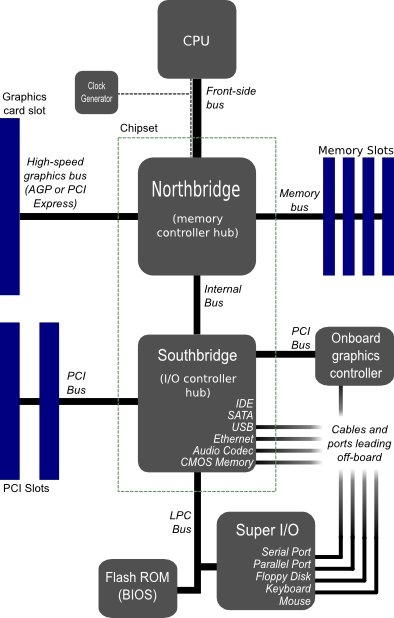
\includegraphics[keepaspectratio,width=0.5\paperwidth]{Pictures/Motherboard_diagram.jpg}
\caption{典型的PC主板}
\label{fig:mainboard}
\end{figure}
某些带有L2和L3缓存(Cache)的计算机,通过后端总线(Back Side Bus)实现这些缓存和中央处理器的连接,而此总线的数据传输速率总是高于前端总线。

大多数现代总线(GTL+和EV6)是CPU和芯片组的连接主干。芯片组(通常由南桥和北桥组成)是和系统中其他总线的连接节点。PCI、AGP和内存总线均和芯片组相连,以使设备间数据能相互传送。

这些第二级系统总线的运行速率取决于前端总线的速率。总之,高的前端总线速率意味着计算机的高处理性能。

在PC发展初期,由于处理器速度不高,大部份元件的时脉均保持同步,直至80486时代,在处理器制程持续进步下,处理器速度也加速成长,当时由于其他外部元件受电气结构所限,而无法跟进成长,因此Intel首次于处理器时脉中加入倍频设计,首颗处理器为Intel 80486DX2,外部传输时脉是处理器的一半,及后处理器成长速度仍远超过外部元件,两者速度差距越来越大。直至Pentium III时代,处理器时脉已超越1GHz,但外部传输时脉仍仅有133MHz。

正常来说,外频速度越高代表处理器在同一周期下可读写越多的数据,因此,外频速度很可能会变成系统效能上的瓶颈,为解决处理器带宽不足的问题,Intel于Pentium 4时代加入Quad Pumped Bus架构,使其在同一周期内可传送4笔数据,此举令外部传输时脉不变下,传输效率却可提升四倍。

\subsection{内频与总线速率}
中央处理器的时脉速度(简称内频)由系统总线速率(bus speed)乘上倍频系数决定。例如,一个时脉速度为 700MHz 的处理器,可能运行于 100MHz 的系统总线上。这说明处理器内的时钟倍频器的倍率设置为7,即中央处理器被设定为以7倍于系统总线的速率运行:100 MHz×7 = 700 MHz。通过改变倍频系数或系统总线速率,可以得到不同的时脉速度。以前经常套用的规则认为:时脉速度=外频(前端总线、FSB)*倍频系数。这句话严格来说并不正确。因为现在系统总线、前端总线(外频、FSB)速率不一样。就 Intel CPU 来说,前端总线=系统总线*4。所以,应该说时脉速度=系统总线*倍频系数。大多数主板允许用户通过跳线设置(BIOS)设定倍频或系统总线速率。现在许多处理器制造商预先锁定了处理器的倍频,但可以通过某些手段解锁。对所有的处理器,系统总线速率的适当提高可以增进其处理速率。

系统总线(BusSpeed)与前端总线(FSB、外频)的区别在于,前端总线(FSB、外频)的速度指的是CPU和北桥芯片间总线的速度。而系统总线(BusSpeed)的概念是建立在数位脉冲信号震荡速度基础之上的,也就是说,100MHz系统总线(BusSpeed)特指数位脉冲信号在每秒钟震荡一百万次,它更多的影响了PCI及其他总线的频率。之所以前端总线(FSB、外频)与系统总线(BusSpeed)这两个概念容易混淆,主要的原因是在以前的很长一段时间里,前端总线(FSB、外频)与系统总线(BusSpeed)是相同速率,因此往往直接称系统总线(BusSpeed)为外频,最终造成这样的误会。随着电脑技术的发展,人们发现前端总线频率(外频、FSB)需要高于系统总线(BusSpeed),因此采用了QDR(Quad Date Rate)技术,或者其他类似的技术实现这个目的。这些技术的原理类似于AGP的2X或者4X,它们使得的前端总线(FSB、外频)频率成为系统总线(BusSpeed)的2倍、4倍甚至更高,从此之后系统总线(BusSpeed)和前端总线(FSB、外频)的区别才开始被人们重视起来。



\subsection{HyperTransport}

HyperTransport技术,简称“HT总线”,以前曾被称作“闪电数据传输”(Lightning Data Transport,LDT),是一种高速、双向、低延时、点对点的、串行或者并行的高带宽连接总线技术,于2001年4月2日开始投入使用。旨在提高个人计算机、服务器、嵌入式系统,以及网络和电信设备内集成电路之间的通信速度。该技术有助于减少系统之中的布线数量,从而能够减少系统瓶颈,让当前速度更快的微处理器能够更加有效地在高端多处理器系统中使用系统内存。由HyperTransport联合会(The HyperTransport Consortium)负责改进和发展此技术。AMD和全美达公司把这项技术应用在x86处理器上,而PMC-Sierra、Broadcom(博通)和Raza Microelectronics则把它应用在MIPS(一种RISC微处理器架构)微处理器上;除微处理器应用之外,AMD、NVIDIA、VIA和SiS把它用于PC主板的芯片组;惠普、Sun Microsystems、IBM、和IWill把它用于服务器领域;Cray、Newisys、 和QLogic把它用于高性能计算;CISCO Systems(思科)把它用于路由器领域。应该引起关注的是以上名单中唯独少了半导体巨头Intel,它继续选择使用一种共享的总线架构,但在Intel新的Nehalem架构(如Core i7)中内置了内存控制器。


具体应用有:
\begin{description}
	\item[替代前端总线]The primary use for HyperTransport is to replace the front-side bus, which is currently different for every type of machine. For instance, a Pentium cannot be plugged into a PCI Express bus. To expand the system, the proprietary front-side bus must connect through adapters for the various standard buses, like AGP or PCI Express. These are typically included in the respective controller functions, namely the northbridge and southbridge.

		In contrast, HyperTransport is an open specification, published by a multi-company consortium. A single HyperTransport adapter chip will work with a wide spectrum of HyperTransport enabled microprocessors. For example, Broadcom HT-1000 and HT-2000 server controller devices can work with many different HyperTransport enabled microprocessors.

		AMD uses HyperTransport to replace the front-side bus in their Opteron, Athlon 64, Sempron 64, Turion 64, Phenom, Phenom II and FX families of microprocessors.
	\item[多处理器]Another use for HyperTransport is as an interconnect for NUMA multiprocessor computers. AMD uses HyperTransport with a proprietary cache coherency extension as part of their Direct Connect Architecture in their Opteron and Athlon 64 FX (Dual Socket Direct Connect (DSDC) Architecture) line of processors. The HORUS interconnect from Newisys extends this concept to larger clusters. The Aqua device from 3Leaf Systems virtualizes and interconnects CPUs, memory, and I/O.
	\item[路由器和交换机]
	\item[协处理器连接]
	\item[扩展设备]
\end{description}


\begin{figure}[htb]
\centering
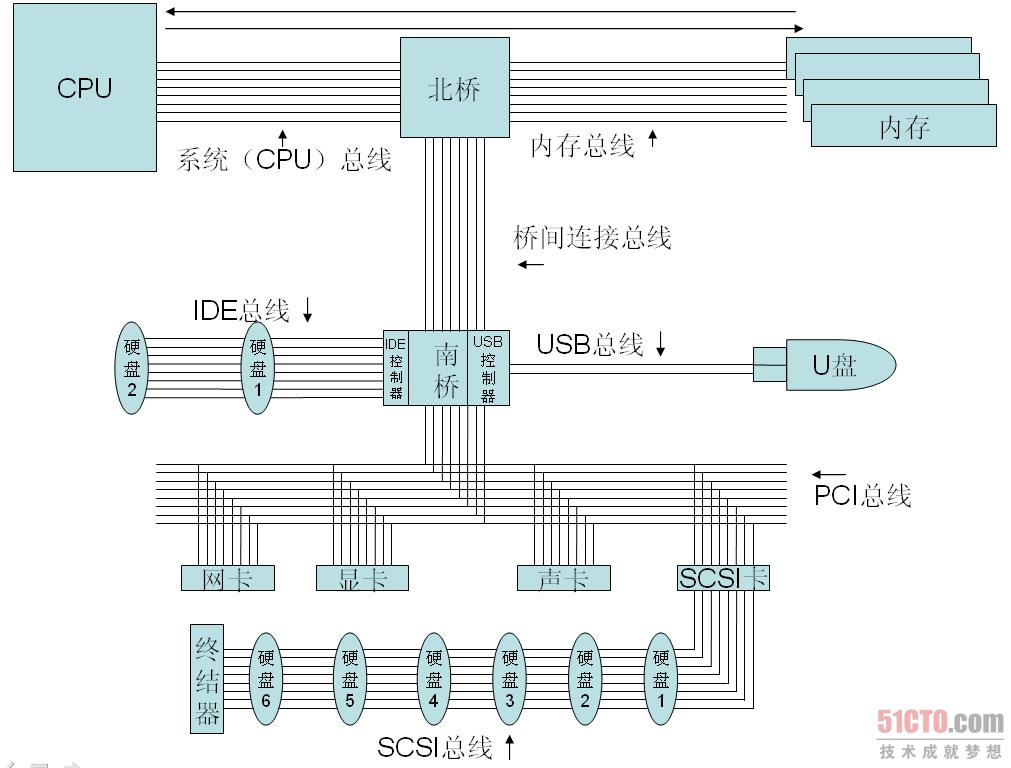
\includegraphics[keepaspectratio,width=0.5\paperwidth]{Pictures/g.jpg}
\caption{计算机总线图}
\label{fig:computerbuspic}
\end{figure}


\subsection{已过时的CNR插槽}
Communications and Networking Riser (CNR) is a slot found on certain PC motherboards and used for specialized networking, audio, and telephony equipment. A motherboard manufacturer can choose to provide audio, networking, or modem functionality in any combination on a CNR card. CNR slots were once commonly found on Pentium 4-class motherboards, but have since been phased out in favor of on-board or embedded components.














